%\chapter{Experimentos e Resultados}
\chapter{Experiments and Results}
\label{chapter:resultados}

%\section{O Aplicativo \textbf{OLAC}}
\section{The Applicative \textbf{OLAC}}

%\par
%Algumas informa��es sobre o aplicativo (linguagem, n�mero de linhas, op��es de execu��o (--help), %\par
%Mostrar gr�fico de ortogonalidade? (m�trica x acur�cia)
%\par
%Mostrar tabela de acertos?
%\par
%O algoritmo n�o ortogonal est� quase igual ao lazy - talvez ele nem precise ser citado
%\par

The applicative \textbf{OLAC} contains the implementation of an association-rule based classifier with three different approaches.
\par
The first one, called \textbf{LAC}, is the classical (and non-orthogonal) \textit{lazy} associative approach  as it was proposed in \cite{Veloso06Lazy}, that just obtains the frequent patterns set and generates rules with it. After that, it chooses the more indicated class according to the rules contained in a rank considering confidence, support and some other metrics.
\par
The second one, called \textbf{OLAC} is  the orthogonal \textit{lazy} associative aproach that obtains an orthogonal set of patterns from the frequent patterns, and generates rules from that pattern set. After that, it chooses the more indiated class the same way it is done with the non-orthogonal approach.
\par
The third one, called \textbf{ORIGAMI} is an implementation of ORIGAMI (as it was proposed in \cite{zaki07origami}) according to the addaptation show in section \ref{sec:ortogonalidade_origami_adaptacao}.
\par
The execution options are shown below:

\begin{verbatim}
Usage: ./olac [options]
Options:
  -i, --training-file       Set the training file
  -t, --testing-file        Set the testing file
  -s, --support             Set the support
  -c, --confidence          Set the confidence
  -r, --run-mode            Set the run mode [c,o] [CLASSICAL, ORTHOGONAL]
  -p, --pattern-set         Set the pattern set type [f,m,r] [FREQUENT,
                              MAXIMAL, RANDOM MAXIMAL]
  -n, --min-num-rules       Set the minimum number of rules
  -l, --max-num-rank-rules  Set the maximum number of rules considered in
                              rank (rank size)
  -m, --min-rule-len        Set the minimum length of the rules
  -x, --max-rule-len        Set the maximum length of the rules
  -o, --orth-mode           Set the orthogonality mode [h,p,o] [HEURISTICAL,
                              POLYNOMIAL, ORIGAMI]
  -e, --orth-metric         Set the orthogonality metric [s,c,l,a]
                              [SIMILARITY, TRANSACTION COVERAGE, CLASS
                              COVERAGE, ALL]
  -w, --orth-method         Set the way metrics are used [s,p,a] [SET, PAIR
                              AVERAGE, ALL]
  -g, --orth-pat-ordering   Set the way patterns are ordered for heuristic
                              [s,r,i,z,n] [SORTED, REVERSE SORTED, SORTED BY
                              SIZE, REVERSE SORTED BY SIZE, NONE]
  -a, --origami-alpha       Set the alpha parameter used by ORIGAMI
  -b, --origami-beta        Set the beta parameter used by ORIGAMI
  -d, --debug               Set the level of debug [0-4] [NODEBUG - MAXLEVEL]
  -v, --verbose             Use verbose mode
  -h, --help                Display this information
\end{verbatim}

The options \textbf{-i} and \textbf{-t} are used to give training and testing files. Support for frquent patter mining and confidence for association rule generation are given by \textbf{s} and \textbf{c}. The option \textbf{-r} is used to choose the running mode (classical, for LAC and orthogonal for OLAC and ORIGAMI). Option \textbf{-p} is used to choose the set of patterns that should be mined by the application. Basically, frequent patterns are used by LAC and OLAC versions, and random maximal frequent patterns are used by ORIGAMI, but it is possible to run \textbf{olac} with different combinations of approaches and pattern sets. The \textbf{-n} options is used to give the minimum number of rules. If it is not possible to generate a minimum number of rules according to the confidence parameter, \textbf{olac} tries to generate rules with lower confidences until this threshold is reached. The \textbf{-l} parameter is used to give the maximum ranking size. The options \textbf{-m} and \textbf{-x} are used to set minimum and maximum number of items in the left side of the rules. The orthogonality mode is given by \textbf{-o}. The used may choose the heuristical mode (OLAC), the polynomial mode (a very expensive approach, that tries all combinations for each set explored), and the ORIGAMI mode. The option \textbf{-e} is used to set the orthogonality metric used by orthogonal modes. The options \textbf{-w} and \textbf{-g} are used to give the way metrics are used and the way patterns are ordered for heauristical mode. The options \textbf{-a} and \textbf{-b} are $\alpha$ and $\beta$, parameters for ORIGAMI approach.

\section{Execution Example}

An example to demonstrate the OLAC execution:

The training data set of table \ref{tab:example_training_db} was created over the set of items $\I = \left\{ A, B, C, D, E \right\}$

\begin{table}[htbp]
	\centering
		\begin{tabular}{|c|c|l|}
		\hline
		\textbf{TID}	& \textbf{Class}	& \textbf{Itemset}	\\
		\hline
		$1$		& $CLASS=1$		& $AB$			\\
		\hline
		$2$		& $CLASS=2$		& $ABC$			\\
		\hline
		$3$		& $CLASS=1$		& $ABD$			\\
		\hline
		$4$		& $CLASS=1$		& $ABDE$		\\
		\hline
		$5$		& $CLASS=1$		& $ABE$			\\
		\hline
		$6$		& $CLASS=3$		& $ADE$			\\
		\hline
		$7$		& $CLASS=2$		& $BC$			\\
		\hline
		$8$		& $CLASS=2$		& $BCD$			\\
		\hline
		$9$		& $CLASS=2$		& $BCE$			\\
		\hline
		$10$		& $CLASS=3$		& $DE$			\\
		\hline
		\end{tabular}
	\caption{Base de Dados de Treinamento para Exemplo}
	\label{tab:example_training_db}
\end{table}


And a testing data set with the transaction $ABE$ and class $CLASS=1$ was used in the test. The applicative \textbf{olac} was first executed with \textbf{LAC} (or non-orthogonal) mode using the parameters found in table \ref{tab:example_run_parms}.

\begin{table}[htbp]
	\centering
		\begin{tabular}{|l|c|}
		\hline
		\textbf{Parameter}	& \textbf{Value}	\\
		\hline
		support			& 0.1			\\
		\hline
		confidence		& 0.1			\\
		\hline
		min-num-rules		& 1			\\
		\hline
		max-num-rank-rules	& 1000			\\
		\hline
		min-rule-len		& 1			\\
		\hline
		max-rule-len		& 1000			\\
		\hline
		\end{tabular}
	\caption{Parameters for non-ortogonal Running Example}
	\label{tab:example_run_parms}
\end{table}

\clearpage

%n�o-ortogonal: 
%accuracy [1], average patterns [7], average rules [15], average time [0.000428]
%padr�es:
%A
%B
%E
%A B
%A E
%B E
%A B E
This execution generated the frequent pattern set $\F = \left\{ A, B, E, AB, AE, BE, ABE \right\}$ and classified correctly the instance. After that, the applicative was executed in \textbf{OLAC} (or orthogonal) mode using the same parameters found in table \ref{tab:example_run_parms}, and similarity as the orthogonality metric. This approach extracted the orthogonal pattern set $\Or = \left\{ AE, B \right\}$ from the frequent pattern set and still classified correctly the instance. As we can see, the set of patterns used by orthogonal mode is much smaller than the original set of frequent patterns. And more, the orthogonal set doesn't have redundancy. It is expected that the redundancy of orthogonal pattern sets are lower than the redundancy of original frequent pattern sets.
\par
%ortogonal - similarity (reverse sorted by side):
%accuracy [1], average patterns [2], average rules [4], average time [0.001799]
%padr�es:
%A E
%B
%
%ortogonal - coverage (sorted):
%accuracy [1], average patterns [2], average rules [5], average time [0.003535]
%padr�es:
%A B
%E
%
%ortogonal - class coverage (sorted by side):
%accuracy [1], average patterns [2], average rules [5], average time [0.003621]
%padr�es:
%B
%E
The applicative was executed with transaction coverage and class coverage as the orthogonality metrics too, extracting, respectively, $\Or = \left\{ AB, E \right\}$ and $\Or = \left\{ B, E \right\}$ as orthogonal pattern sets, and these executions classified the instance correctly too.

\section{Experiments}

Now, we will show some graphics comparing the executions of the three approaches implemented: LAC, OLAC and ORIGAMI. %, but first we will do some observations about these test instances:
%\par
%\begin{itemize}
%	\item LAC was run with support 1, just because this is the objective of LAC (the Adriano Veloso implementation) - to get better results with the minimum support value;
%	\item ORIGAMI was run with $\alpha = 0.2$, and $\beta = 0.8$, we need to make more tests with another values for $\alpha$ and $\beta$ in order to get better results;
%	\item We are still running these experiments with anoter parameters, and trying to get some better results for all approaches.
%\end{itemize}
\par
The figure \ref{fig:histogram_best_run_for_each_db_acc} shows a histogram with the best accuracies for each dataset obtained with the three approaches. The figure \ref{fig:histogram_best_run_for_each_db_pat} shows a histogram with the average number of patterns used for each classification, the figure \ref{fig:histogram_best_run_for_each_db_rul} shows the average number of rules generated for each classification, and the figure \ref{fig:histogram_best_run_for_each_db_tim} shows the average time spent for each classification. For these four results it was used the best sets of parameters for each application and dataset, for example, considering the orthogonal classifier OLAC, for anneal.ac we used support equals to 0.001, but for waveform.ac we used support equals to 0.0001, since the best results were obtained with this value.

\begin{figure}[htbp]
	\centering
	\includegraphics[width=0.95\textwidth]{graphs/histogram_best_run_for_each_db_acc}
	\caption{Accuracy Histogram (best results for each dataset)}
	\label{fig:histogram_best_run_for_each_db_acc}
\end{figure}

As we can see in the figure \ref{fig:histogram_best_run_for_each_db_acc}, the accuracies for orthogonal and non-orthogonal versions of our classifier are very close. the average accuracy obtained for them were $0.8085$ and $0.8088$ respectively, and they are both better than LAC.

\begin{figure}[htbp]
	\centering
	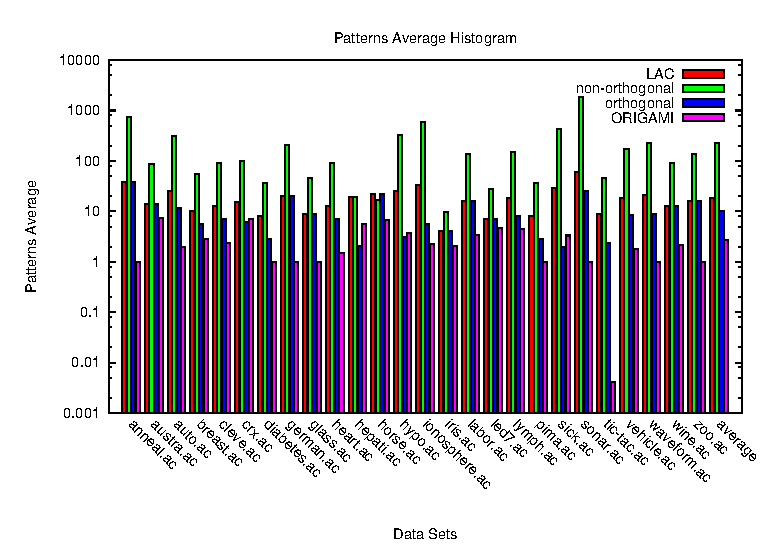
\includegraphics[width=0.95\textwidth]{graphs/histogram_best_run_for_each_db_pat}
	\caption{Patterns Histogram (best results for each dataset)}
	\label{fig:histogram_best_run_for_each_db_pat}
\end{figure}

The number of patterns generated by orthogonal version of our classifier (shown by figure \ref{fig:histogram_best_run_for_each_db_pat}) is lower than the LAC ones. The difference would be still greater (as it was comparing our orthogonal and non-orthogonal versions) if we used lower values for confidence in LAC (the value for this parameter that produced better results in average was $0.95$.

\begin{figure}[htbp]
	\centering
	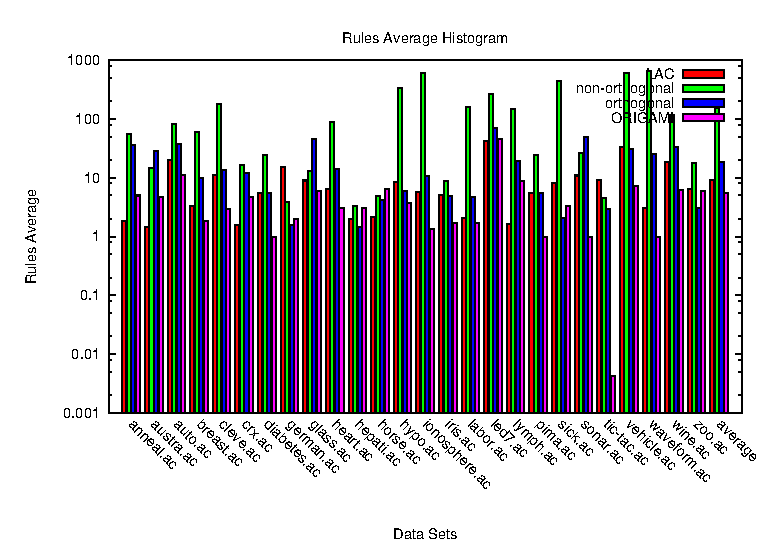
\includegraphics[width=0.95\textwidth]{graphs/histogram_best_run_for_each_db_rul}
	\caption{Rules Histogram (best results for each dataset)}
	\label{fig:histogram_best_run_for_each_db_rul}
\end{figure}

The number of patterns generated by orthogonal version of our classifier (shown by figure \ref{fig:histogram_best_run_for_each_db_rul}) is higher than the LAC ones. This happened because the same - the values for confidence used for LAC were very high. We believe that if we run LAC with lower values for confidence, this number will be much higher.

\begin{figure}[htbp]
	\centering
	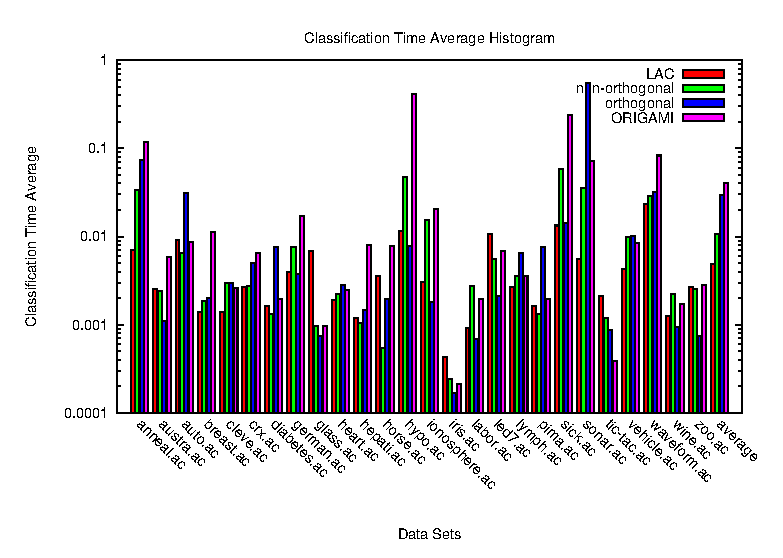
\includegraphics[width=0.95\textwidth]{graphs/histogram_best_run_for_each_db_tim}
	\caption{Classification Time Histogram (best results for each dataset)}
	\label{fig:histogram_best_run_for_each_db_tim}
\end{figure}

\clearpage

The table \ref{tab:best_runs_for_each_db_lac} shows the parameters used LAC and the best results for each dataset.

\begin{table}[htbp]
	\centering
		\begin{tabular}{|l|c|c|c|c|c|c|c|c|c|c|}
		\hline
		\textbf{dataset}	& \textbf{s}	& \textbf{c}	& \textbf{n}	& \textbf{l}	& \textbf{m}	& \textbf{x}	& \textbf{pat.}	& \textbf{rul.}	& \textbf{t.}	& \textbf{acc.}	\\
		\hline
		anneal.ac      & 0.001    & 0.7         & 1              & 1000                & 1             & 1             & 37.995         & 36.544         & 0.002          & 0.914          \\
		\hline
		austra.ac      & 0.1      & 0.8         & 1              & 100                 & 1             & 2             & 85.825         & 14.458         & 0.002          & 0.861          \\
		\hline
		auto.ac        & 0.01     & 0.8         & 1              & 10                  & 1             & 2             & 298.140        & 48.891         & 0.006          & 0.518          \\
		\hline
		breast.ac      & 0.1      & 0.0001      & 1              & 100                 & 1             & 1             & 9.661          & 19.322         & 0.001          & 0.960          \\
		\hline
		cleve.ac       & 0.0001   & 0.0001      & 1              & 100                 & 1             & 1             & 13.000         & 25.987         & 0.001          & 0.808          \\
		\hline
		crx.ac         & 0.1      & 0.8         & 1              & 1000                & 1             & 2             & 97.784         & 16.925         & 0.003          & 0.864          \\
		\hline
		diabetes.ac    & 0.01     & 0.6         & 1              & 100                 & 1             & 2             & 35.993         & 24.767         & 0.001          & 0.776          \\
		\hline
		german.ac      & 0.01     & 0.9         & 1              & 10                  & 1             & 2             & 207.909        & 3.714          & 0.007          & 0.724          \\
		\hline
		glass.ac       & 0.01     & 0.6         & 1              & 1000                & 1             & 2             & 44.884         & 12.829         & 0.001          & 0.710          \\
		\hline
		heart.ac       & 0.2      & 0.3         & 1              & 1000                & 1             & 2             & 83.326         & 118.570        & 0.002          & 0.830          \\
		\hline
		hepati.ac      & 0.1      & 0.5         & 1              & 1                   & 1             & 1             & 18.437         & 18.437         & 0.000          & 0.846          \\
		\hline
		horse.ac       & 0.3      & 0.5         & 1              & 100                 & 1             & 2             & 59.599         & 59.596         & 0.002          & 0.813          \\
		\hline
		hypo.ac        & 0.1      & 0.99        & 1              & 10                  & 1             & 2             & 290.838        & 56.591         & 0.042          & 0.978          \\
		\hline
		ionosphere.ac  & 0.01     & 0.4         & 1              & 1000                & 1             & 2             & 568.612        & 594.367        & 0.014          & 0.923          \\
		\hline
		iris.ac        & 0.1      & 0.3         & 1              & 10                  & 1             & 2             & 9.467          & 10.467         & 0.000          & 0.967          \\
		\hline
		labor.ac       & 0.3      & 0.9         & 1              & 10                  & 1             & 2             & 54.027         & 6.177          & 0.001          & 0.933          \\
		\hline
		led7.ac        & 0.1      & 0.0001      & 1              & 1000                & 1             & 2             & 27.311         & 271.501        & 0.006          & 0.729          \\
		\hline
		lymph.ac       & 0.01     & 0.5         & 1              & 1000                & 1             & 2             & 168.905        & 167.611        & 0.004          & 0.796          \\
		\hline
		pima.ac        & 0.0001   & 0.7         & 1              & 10                  & 1             & 1             & 8.000          & 3.270          & 0.000          & 0.753          \\
		\hline
		sick.ac        & 0.0001   & 0.4         & 1              & 1                   & 1             & 1             & 28.999         & 28.999         & 0.006          & 0.968          \\
		\hline
		sonar.ac       & 0.01     & 0.9         & 1              & 100                 & 1             & 2             & 1829.861       & 29.219         & 0.031          & 0.784          \\
		\hline
		tic-tac.ac     & 0.0001   & 0.5         & 1              & 1                   & 1             & 1             & 9.000          & 9.000          & 0.001          & 0.710          \\
		\hline
		vehicle.ac     & 0.0001   & 0.0001      & 1              & 100                 & 1             & 1             & 18.000         & 68.306         & 0.001          & 0.592          \\
		\hline
		waveform.ac    & 0.0001   & 0.0001      & 1              & 100                 & 1             & 1             & 21.000         & 62.912         & 0.006          & 0.765          \\
		\hline
		wine.ac        & 0.01     & 0.3         & 1              & 1000                & 1             & 2             & 90.577         & 118.375        & 0.002          & 0.994          \\
		\hline
		zoo.ac         & 0.001    & 0.7         & 1              & 1000                & 1             & 1             & 15.990         & 2.674          & 0.000          & 0.650          \\
		\hline
		\end{tabular}
	\caption{Best Parameters and Results for each Dataset (for LAC)}
	\label{tab:best_runs_for_each_db_lac}
\end{table}

\clearpage

The table \ref{tab:best_runs_for_each_db_olac} shows the parameters used OLAC and the best results for each dataset.

\begin{table}[htbp]
	\centering
		\begin{tabular}{|l|c|c|c|c|c|c|c|c|c||c|c|c|c|}
		\hline
		\textbf{dataset}	& \textbf{s}	& \textbf{c}	& \textbf{n}	& \textbf{l}	& \textbf{m}	& \textbf{x}	& \textbf{e} & \textbf{w} & \textbf{g} & \textbf{pat.}	& \textbf{rul.}	& \textbf{t.}	& \textbf{acc.}	\\
		\hline
		anneal.ac      & 0.0001   & 0.8         & 1              & 1000                & 1             & 2             & s      & s        & s        & 21.27          & 5.64           & 0.20           & 0.92           \\
		\hline
		austra.ac      & 0.3      & 0.7         & 1              & 10                  & 1             & 2             & s      & s        & n        & 11.28          & 3.01           & 0.00           & 0.86           \\
		\hline
		auto.ac        & 0.01     & 0.4         & 1              & 10                  & 1             & 1             & s      & s        & n        & 24.25          & 12.12          & 0.00           & 0.52           \\
		\hline
		breast.ac      & 0.0001   & 0.0001      & 1              & 10                  & 1             & 2             & s      & s        & r        & 4.88           & 9.51           & 0.00           & 0.97           \\
		\hline
		cleve.ac       & 0.01     & 0.3         & 1              & 1000                & 1             & 2             & s      & s        & s        & 8.59           & 12.25          & 0.00           & 0.84           \\
		\hline
		crx.ac         & 0.3      & 0.7         & 1              & 10                  & 1             & 3             & s      & p        & n        & 12.00          & 3.00           & 0.05           & 0.86           \\
		\hline
		diabetes.ac    & 0.0001   & 0.0001      & 1              & 10                  & 1             & 2             & c      & s        & n        & 2.93           & 5.86           & 0.01           & 0.76           \\
		\hline
		german.ac      & 0.0001   & 0.8         & 1              & 1000                & 1             & 2             & s      & s        & s        & 12.35          & 1.60           & 0.02           & 0.72           \\
		\hline
		glass.ac       & 0.1      & 0.01        & 1              & 100                 & 1             & 2             & s      & s        & s        & 6.54           & 31.88          & 0.00           & 0.70           \\
		\hline
		heart.ac       & 0.01     & 0.3         & 1              & 1000                & 1             & 2             & s      & s        & s        & 8.50           & 11.95          & 0.00           & 0.83           \\
		\hline
		hepati.ac      & 0.0001   & 0.3         & 1              & 100                 & 1             & 1             & c      & s        & s        & 2.03           & 2.59           & 0.00           & 0.86           \\
		\hline
		horse.ac       & 0.3      & 0.7         & 1              & 10                  & 1             & 2             & s      & s        & n        & 13.11          & 1.29           & 0.01           & 0.81           \\
		\hline
		hypo.ac        & 0.0001   & 0.99        & 1              & 10                  & 1             & 1             & s      & p        & z        & 25.00          & 3.13           & 0.01           & 0.98           \\
		\hline
		ionosphere.ac  & 0.001    & 0.3         & 1              & 100                 & 1             & 1             & s      & s        & s        & 34.00          & 40.34          & 0.01           & 0.91           \\
		\hline
		iris.ac        & 0.01     & 0.3         & 1              & 1000                & 1             & 2             & s      & s        & s        & 3.61           & 4.32           & 0.00           & 0.97           \\
		\hline
		labor.ac       & 0.1      & 0.6         & 1              & 10                  & 1             & 2             & s      & s        & z        & 9.44           & 8.25           & 0.00           & 0.93           \\
		\hline
		led7.ac        & 0.0001   & 0.0001      & 1              & 100                 & 1             & 1             & s      & s        & s        & 7.00           & 70.00          & 0.00           & 0.63           \\
		\hline
		lymph.ac       & 0.01     & 0.6         & 1              & 10                  & 1             & 2             & s      & s        & s        & 8.79           & 4.44           & 0.01           & 0.78           \\
		\hline
		pima.ac        & 0.0001   & 0.4         & 1              & 100                 & 1             & 5             & l      & s        & r        & 4.80           & 6.11           & 0.03           & 0.76           \\
		\hline
		sick.ac        & 0.001    & 0.2         & 1              & 100                 & 1             & 2             & c      & s        & s        & 3.26           & 3.48           & 0.46           & 0.96           \\
		\hline
		sonar.ac       & 0.01     & 0.5         & 1              & 100                 & 1             & 2             & l      & s        & s        & 3.82           & 3.82           & 0.06           & 0.79           \\
		\hline
		tic-tac.ac     & 0.01     & 0.7         & 1              & 10                  & 1             & 5             & l      & s        & z        & 7.89           & 5.07           & 0.04           & 0.80           \\
		\hline
		vehicle.ac     & 0.0001   & 0.0001      & 1              & 100                 & 1             & 2             & s      & s        & z        & 8.00           & 27.95          & 0.02           & 0.64           \\
		\hline
		waveform.ac    & 0.0001   & 0.0001      & 1              & 100                 & 1             & 2             & s      & s        & r        & 9.58           & 27.32          & 0.06           & 0.79           \\
		\hline
		wine.ac        & 0.0001   & 0.0001      & 1              & 100                 & 1             & 2             & s      & s        & z        & 8.96           & 20.94          & 0.00           & 0.96           \\
		\hline
		zoo.ac         & 0.01     & 0.6         & 1              & 10                  & 1             & 2             & s      & s        & s        & 8.36           & 3.38           & 0.00           & 0.73           \\
		\hline
		\end{tabular}
	\caption{Best Parameters and Results for each Dataset (for OLAC)}
	\label{tab:best_runs_for_each_db_olac}
\end{table}

\clearpage

The table \ref{tab:best_runs_for_each_db_origami} shows the parameters used ORIGAMI and the best results for each dataset.

\begin{table}[htbp]
	\centering
		\renewcommand{\tabcolsep}{1.8mm}
		\begin{tabular}{|l|c|c|c|c|c|c|c|c||c|c|c|c|}
		\hline
		\textbf{dataset}	& \textbf{s}	& \textbf{c}	& \textbf{n}	& \textbf{l}	& \textbf{u}	& \textbf{e} & \textbf{a} & \textbf{b} & \textbf{pat.}	& \textbf{rul.}	& \textbf{tim.}	& \textbf{acc.}	\\
		\hline
		anneal.ac      & 0.0001   & 0.0001      & 1              & 10       & c                   & s        & 0.7    & 0.9   & 1.01           & 1.01           & 0.02           & 0.96           \\
		\hline
		austra.ac      & 0.1      & 0.0001      & 1              & 100      & c                   & s        & 0.7    & 0.8   & 30.35          & 60.62          & 0.03           & 0.87           \\
		\hline
		auto.ac        & 0.1      & 0.0001      & 1              & 100      & c                   & s        & 0.7    & 0.8   & 13.47          & 51.30          & 0.02           & 0.56           \\
		\hline
		breast.ac      & 0.0001   & 0.0001      & 1              & 10       & o                   & s        & 0.1    & 0.5   & 1.00           & 1.01           & 0.00           & 0.96           \\
		\hline
		cleve.ac       & 0.1      & 0.0001      & 1              & 100      & c                   & s        & 0.7    & 0.8   & 14.76          & 28.91          & 0.01           & 0.84           \\
		\hline
		crx.ac         & 0.1      & 0.0001      & 1              & 100      & c                   & s        & 0.7    & 0.8   & 27.52          & 54.99          & 0.03           & 0.86           \\
		\hline
		diabetes.ac    & 0.1      & 0.0001      & 1              & 10       & k                   & s        & 0.7    & 0.8   & 4.49           & 8.97           & 0.00           & 0.79           \\
		\hline
		german.ac      & 0.1      & 0.0001      & 1              & 10       & e                   & c        & 0.2    & 0.8   & 8.03           & 16.05          & 0.11           & 0.73           \\
		\hline
		glass.ac       & 0.0001   & 0.0001      & 1              & 10       & c                   & s        & 0.1    & 0.5   & 1.00           & 2.00           & 0.00           & 0.77           \\
		\hline
		heart.ac       & 0.1      & 0.0001      & 1              & 10       & e                   & s        & 0.2    & 0.8   & 1.00           & 1.90           & 0.00           & 0.84           \\
		\hline
		hepati.ac      & 0.001    & 0.001       & 1              & 100      & s                   & s        & 0.1    & 0.8   & 1.00           & 1.00           & 0.00           & 0.88           \\
		\hline
		horse.ac       & 0.1      & 0.5         & 1              & 100      & c                   & s        & 0.7    & 0.8   & 53.77          & 54.63          & 0.11           & 0.79           \\
		\hline
		hypo.ac        & 0.0001   & 0.0001      & 1              & 10       & c                   & s        & 0.3    & 0.5   & 1.00           & 1.04           & 0.03           & 0.98           \\
		\hline
		ionosphere.ac  & 0.1      & 0.0001      & 1              & 100      & c                   & s        & 0.7    & 0.8   & 27.71          & 49.06          & 0.29           & 0.89           \\
		\hline
		iris.ac        & 0.1      & 0.0001      & 1              & 10       & n                   & s        & 0.2    & 0.8   & 1.06           & 1.37           & 0.00           & 0.95           \\
		\hline
		labor.ac       & 0.0001   & 0.001       & 1              & 1        & v                   & s        & 0.2    & 0.6   & 1.07           & 1.07           & 0.00           & 0.95           \\
		\hline
		led7.ac        & 0.001    & 0.0001      & 1              & 10       & c                   & l        & 0.1    & 0.4   & 1.04           & 4.56           & 0.00           & 0.73           \\
		\hline
		lymph.ac       & 0.1      & 0.001       & 1              & 100      & n                   & s        & 0.6    & 0.7   & 18.25          & 37.23          & 0.03           & 0.84           \\
		\hline
		pima.ac        & 0.1      & 0.0001      & 1              & 10       & l                   & s        & 0.7    & 0.9   & 4.52           & 9.03           & 0.00           & 0.78           \\
		\hline
		sick.ac        & 0.0001   & 0.0001      & 1              & 10       & c                   & s        & 0.2    & 0.7   & 1.00           & 1.14           & 0.03           & 0.97           \\
		\hline
		sonar.ac       & 0.1      & 0.0001      & 1              & 10       & i                   & s        & 0.2    & 0.9   & 1.00           & 1.81           & 0.32           & 0.83           \\
		\hline
		tic-tac.ac     & 0.0001   & 0.0001      & 1              & 1        & c                   & s        & 0.2    & 0.7   & 1.01           & 1.02           & 0.00           & 0.82           \\
		\hline
		vehicle.ac     & 0.0001   & 0.0001      & 1              & 10       & c                   & s        & 0.2    & 0.8   & 1.01           & 1.12           & 0.00           & 0.69           \\
		\hline
		waveform.ac    & 0.01     & 0.0001      & 1              & 100      & c                   & s        & 0.7    & 0.8   & 87.71          & 214.78         & 0.97           & 0.76           \\
		\hline
		wine.ac        & 0.0001   & 0.0001      & 1              & 1        & c                   & s        & 0.1    & 0.7   & 1.02           & 1.02           & 0.00           & 0.94           \\
		\hline
		zoo.ac         & 0.0001   & 0.6         & 1              & 10       & p                   & s        & 0.3    & 0.7   & 1.02           & 1.02           & 0.00           & 0.84           \\
		\hline
		\end{tabular}
	\caption{Melhores Par�metros e Resultados para Cada Base de Dados (ORIGAMI)}
	\label{tab:best_runs_for_each_db_origami}
\end{table}


\clearpage

The figure \ref{fig:histogram_best_run_for_avg_db_acc} shows a histogram with the best accuracies for each dataset obtained with LAC, ORIGAMI, orthogonal classifier and non-orthogonal classifier. The figure \ref{fig:histogram_best_run_for_avg_db_pat} shows a histogram with the average number of patterns used for each classification, the figure \ref{fig:histogram_best_run_for_avg_db_rul} shows the average number of rules generated for each classification and the figure \ref{fig:histogram_best_run_for_avg_db_tim} shows the average spent for each classification. For those three results it was used, for each application, the set of parameters that produced the best average accuracy for the whole set of data. The values for each parameter are shown in table \ref{tab:best_parms_for_avg_db}. Some parameters are not applicable to all approaches.

\begin{table}[htbp]
	\centering
		\begin{tabular}{|l|c|c|c|}
		\hline
					& \textbf{LAC}	& \textbf{OLAC}	& \textbf{ORIGAMI}	\\
		\hline
		support			& 0.01		& 0.01		& 0.1			\\
		\hline
		confidence		& 0.6		& 0.001		& 0.0001		\\
		\hline
		min-num-rules		& 1		& 1		& 1			\\
		\hline
		max-num-rank-rules	& 1000		& 100		& 1000			\\
		\hline
		min-rule-len		& 1		& 1		& -			\\
		\hline
		max-rule-len		& 2		& 2		& -			\\
		\hline
		metric			& -		& s		& s			\\
		\hline
		method			& -		& s		& -			\\
		\hline
		pat-ordering		& -		& s		& -			\\
		\hline
		alpha			& -		& -		& 0.7			\\
		\hline
		beta			& -		& -		& 0.8			\\
		\hline
		\end{tabular}
	\caption{Best Parameters for Each Run}
	\label{tab:best_parms_for_avg_db}
\end{table}


\begin{figure}[htbp]
	\centering
	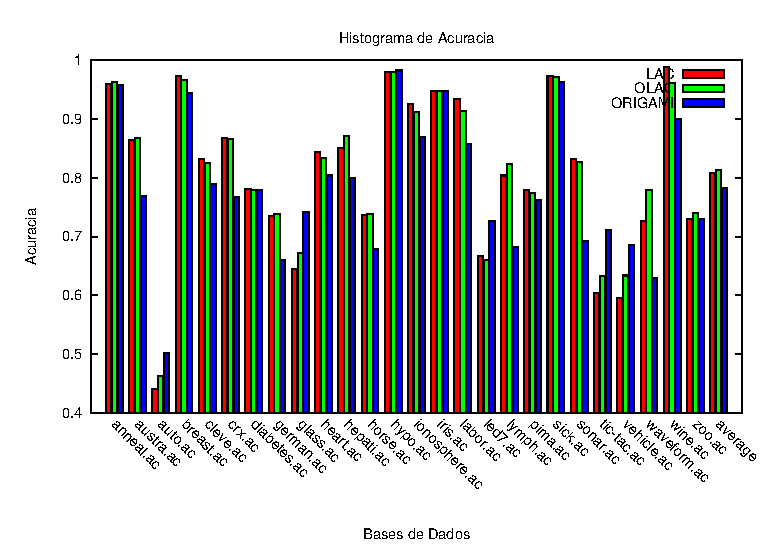
\includegraphics[width=0.95\textwidth]{graphs/histogram_best_run_for_avg_db_acc}
	\caption{Accuracy Histogram (best average results for all datasets)}
	\label{fig:histogram_best_run_for_avg_db_acc}
\end{figure}

\begin{figure}[htbp]
	\centering
	\includegraphics[width=0.95\textwidth]{graphs/histogram_best_run_for_avg_db_pat}
	\caption{Patterns Histogram (best average results for all datasets)}
	\label{fig:histogram_best_run_for_avg_db_pat}
\end{figure}

The number of patterns generated with ORIGAMI approach in figure \ref{fig:histogram_best_run_for_avg_db_pat} was $1$ (one) for all datasets. This happened because the best combined values for support and confidence found was $0.001$ and $0.1$, and this, possibly, didn't generate any valid rule, since the low support generates big maximal patterns, and $0.1$ is a sufficient value for confidence to turn all rules invalid. Since the applicative tries to generate, at least, one rule for each test instance, just one of the rules is added to the result. As it was told before, we are running the experiment with more parameter combinations, searching for better results.

\begin{figure}[htbp]
	\centering
	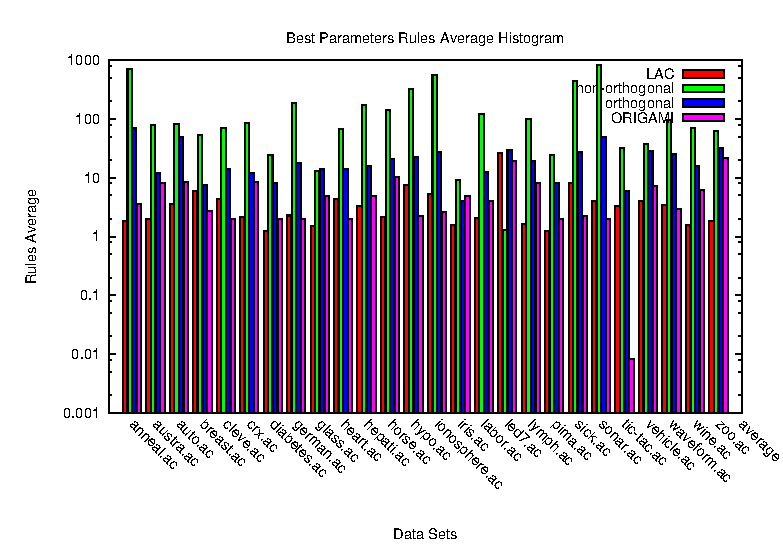
\includegraphics[width=0.95\textwidth]{graphs/histogram_best_run_for_avg_db_rul}
	\caption{Rules Histogram (best average results for all datasets)}
	\label{fig:histogram_best_run_for_avg_db_rul}
\end{figure}

\begin{figure}[htbp]
	\centering
	\includegraphics[width=0.95\textwidth]{graphs/histogram_best_run_for_avg_db_tim}
	\caption{Classification Time Histogram (best average results for all datasets)}
	\label{fig:histogram_best_run_for_avg_db_tim}
\end{figure}

\clearpage

In table \ref{tab:comparison_lac_olac} we have a comparison between the execution of LAC and OLAC approaches. This table shows the number of hits of both (second column), the number of hits of OLAC that LAC didn't get (third column), the number of hits of LAC that OLAC didn't get (fourth column) and the number of instances that both missed.

\begin{table}[htbp]
	\centering
		\begin{tabular}{|l|c|c|c|c|}
		\hline
				& \textbf{OLAC}		& \textbf{OLAC}			& \textbf{$\neg$ OLAC}	& \textbf{$\neg$ OLAC}	\\
		\textbf{Data Sets}	& \textbf{\&}		& \textbf{\&}			& \textbf{\&}			& \textbf{\&}			\\
				& \textbf{LAC}		& \textbf{$\neg$ LAC}		& \textbf{LAC}			& \textbf{$\neg$ LAC}		\\
		\hline
		anneal.ac       & 726           & 5                  & 3                        & 64                            \\
		\hline
		austra.ac       & 573           & 17                 & 21                       & 79                            \\
		\hline
		auto.ac         & 66            & 40                 & 40                       & 59                            \\
		\hline
		breast.ac       & 668           & 7                  & 3                        & 21                            \\
		\hline
		cleve.ac        & 239           & 16                 & 6                        & 42                            \\
		\hline
		crx.ac          & 579           & 11                 & 17                       & 83                            \\
		\hline
		diabetes.ac     & 557           & 26                 & 39                       & 146                           \\
		\hline
		german.ac       & 631           & 89                 & 93                       & 187                           \\
		\hline
		glass.ac        & 131           & 18                 & 21                       & 44                            \\
		\hline
		heart.ac        & 218           & 6                  & 6                        & 40                            \\
		\hline
		hepati.ac       & 120           & 13                 & 11                       & 11                            \\
		\hline
		horse.ac        & 298           & 0                  & 1                        & 69                            \\
		\hline
		hypo.ac         & 3083          & 2                  & 10                       & 68                            \\
		\hline
		ionosphere.ac   & 314           & 4                  & 10                       & 23                            \\
		\hline
		iris.ac         & 145           & 0                  & 0                        & 5                             \\
		\hline
		labor.ac        & 51            & 2                  & 2                        & 2                             \\
		\hline
		led7.ac         & 1988          & 39                 & 346                      & 827                           \\
		\hline
		lymph.ac        & 106           & 10                 & 12                       & 20                            \\
		\hline
		pima.ac         & 535           & 50                 & 43                       & 140                           \\
		\hline
		sick.ac         & 2631          & 49                 & 78                       & 42                            \\
		\hline
		sonar.ac        & 128           & 36                 & 35                       & 9                             \\
		\hline
		tic-tac.ac      & 601           & 167                & 79                       & 111                           \\
		\hline
		vehicle.ac      & 474           & 65                 & 27                       & 280                           \\
		\hline
		waveform.ac     & 3688          & 281                & 135                      & 896                           \\
		\hline
		wine.ac         & 171           & 0                  & 6                        & 1                             \\
		\hline
		zoo.ac          & 64            & 10                 & 2                        & 25                            \\
		\hline
		average         & 722.50        & 37.04              & 40.23                    & 126.69                        \\
		\hline
		\end{tabular}
	\caption{Comparison between LAC and OLAC (number of asserts)}
	\label{tab:comparison_lac_olac}
\end{table}

\clearpage

In table \ref{tab:comparison_lac_origami} we have a comparison between the execution of LAC and ORIGAMI approaches. This table shows the number of hits of both (second column), the number of hits of ORIGAMI that LAC didn't get (third column), the number of hits of LAC that ORIGAMI didn't get (fourth column) and the number of instances that both missed.

\begin{table}[htbp]
	\centering
		\begin{tabular}{|l|c|c|c|c|}
		\hline
				& \textbf{ORIGAMI}	& \textbf{ORIGAMI}		& \textbf{$\neg$ ORIGAMI}	& \textbf{$\neg$ ORIGAMI}	\\
		\textbf{Data Sets}	& \textbf{\&}		& \textbf{\&}			& \textbf{\&}			& \textbf{\&}			\\
				&  \textbf{LAC}		& \textbf{$\neg$ LAC}		& \textbf{LAC}			& \textbf{$\neg$ LAC}		\\
		\hline
		anneal.ac       & 714           & 49                 & 22                       & 13                            \\
		\hline
		austra.ac       & 567           & 35                 & 27                       & 61                            \\
		\hline
		auto.ac         & 60            & 50                 & 46                       & 49                            \\
		\hline
		breast.ac       & 660           & 9                  & 18                       & 12                            \\
		\hline
		cleve.ac        & 245           & 10                 & 5                        & 43                            \\
		\hline
		crx.ac          & 562           & 32                 & 34                       & 62                            \\
		\hline
		diabetes.ac     & 560           & 41                 & 36                       & 131                           \\
		\hline
		german.ac       & 574           & 153                & 150                      & 123                           \\
		\hline
		glass.ac        & 141           & 25                 & 11                       & 37                            \\
		\hline
		heart.ac        & 213           & 13                 & 11                       & 33                            \\
		\hline
		hepati.ac       & 115           & 17                 & 16                       & 7                             \\
		\hline
		horse.ac        & 289           & 3                  & 10                       & 66                            \\
		\hline
		hypo.ac         & 3070          & 42                 & 23                       & 28                            \\
		\hline
		ionosphere.ac   & 310           & 8                  & 14                       & 19                            \\
		\hline
		iris.ac         & 140           & 3                  & 5                        & 2                             \\
		\hline
		labor.ac        & 50            & 3                  & 3                        & 1                             \\
		\hline
		led7.ac         & 2202          & 125                & 132                      & 741                           \\
		\hline
		lymph.ac        & 108           & 12                 & 10                       & 18                            \\
		\hline
		pima.ac         & 554           & 53                 & 34                       & 127                           \\
		\hline
		sick.ac         & 2675          & 45                 & 34                       & 46                            \\
		\hline
		sonar.ac        & 133           & 32                 & 30                       & 13                            \\
		\hline
		tic-tac.ac      & 584           & 204                & 96                       & 74                            \\
		\hline
		vehicle.ac      & 422           & 155                & 97                       & 172                           \\
		\hline
		waveform.ac     & 3355          & 414                & 593                      & 638                           \\
		\hline
		wine.ac         & 174           & 1                  & 3                        & 0                             \\
		\hline
		zoo.ac          & 66            & 13                 & 12                       & 10                            \\
		\hline
		average         & 713.19        & 59.50              & 56.62                    & 97.15                         \\
		\hline
		\end{tabular}
	\caption{Comparison between LAC and ORIGAMI (number of asserts)}
	\label{tab:comparison_lac_origami}
\end{table}

\clearpage

In table \ref{tab:comparison_olac_origami} we have a comparison between the execution of OLAC and ORIGAMI approaches. This table shows the number of hits of both (second column), the number of hits of OLAC that ORIGAMI didn't get (third column), the number of hits of ORIGAMI that OLAC didn't get (fourth column) and the number of instances that 
both missed.

\begin{table}[htbp]
	\centering
		\begin{tabular}{|l|c|c|c|c|}
		\hline
				& \textbf{OLAC}		& \textbf{OLAC}			& \textbf{$\neg$ OLAC}	& \textbf{$\neg$ OLAC}	\\
		\textbf{Data Sets}	& \textbf{\&}		& \textbf{\&}			& \textbf{\&}			& \textbf{\&}			\\
				& \textbf{ORIGAMI}	& \textbf{$\neg$ ORIGAMI}	& \textbf{ORIGAMI}		& \textbf{$\neg$ ORIGAMI}	\\
		\hline
		anneal.ac       & 743           & 25                 & 21                       & 9                             \\
		\hline
		austra.ac       & 503           & 96                 & 28                       & 63                            \\
		\hline
		auto.ac         & 47            & 48                 & 56                       & 54                            \\
		\hline
		breast.ac       & 654           & 21                 & 6                        & 18                            \\
		\hline
		cleve.ac        & 216           & 34                 & 23                       & 30                            \\
		\hline
		crx.ac          & 499           & 98                 & 30                       & 63                            \\
		\hline
		diabetes.ac     & 543           & 55                 & 55                       & 115                           \\
		\hline
		german.ac       & 549           & 189                & 111                      & 151                           \\
		\hline
		glass.ac        & 132           & 12                 & 27                       & 43                            \\
		\hline
		heart.ac        & 201           & 24                 & 16                       & 29                            \\
		\hline
		hepati.ac       & 114           & 21                 & 10                       & 10                            \\
		\hline
		horse.ac        & 209           & 63                 & 41                       & 55                            \\
		\hline
		hypo.ac         & 3080          & 20                 & 27                       & 36                            \\
		\hline
		ionosphere.ac   & 289           & 31                 & 16                       & 15                            \\
		\hline
		iris.ac         & 140           & 2                  & 2                        & 6                             \\
		\hline
		labor.ac        & 46            & 6                  & 3                        & 2                             \\
		\hline
		led7.ac         & 1983          & 130                & 340                      & 747                           \\
		\hline
		lymph.ac        & 91            & 31                 & 10                       & 16                            \\
		\hline
		pima.ac         & 533           & 61                 & 52                       & 122                           \\
		\hline
		sick.ac         & 2673          & 45                 & 25                       & 57                            \\
		\hline
		sonar.ac        & 126           & 46                 & 18                       & 18                            \\
		\hline
		tic-tac.ac      & 474           & 132                & 208                      & 144                           \\
		\hline
		vehicle.ac      & 445           & 91                 & 135                      & 175                           \\
		\hline
		waveform.ac     & 2622          & 1271               & 525                      & 582                           \\
		\hline
		wine.ac         & 156           & 15                 & 4                        & 3                             \\
		\hline
		zoo.ac          & 67            & 8                  & 7                        & 19                            \\
		\hline
		average         & 659.04        & 99.04              & 69.08                    & 99.31                         \\
		\hline
		\end{tabular}
	\caption{Compara��o entre OLAC e ORIGAMI (numero de acertos)}
	\label{tab:comparison_olac_origami}
\end{table}

%\section{Compara��o Ortogonal x N�o Ortogonal}
%
%Histogramas de acur�cia, n�mero de padr�es e n�mero de regras. \\
%Comparar melhor conjunto de par�metros para cada arquivo e melhor conjunto de par�metros para todos os arquivos juntos.
%
%\section{Compara��o Ortogonal x LAC}
%
%Histogramas de acur�cia, n�mero de padr�es e n�mero de regras. \\
%Comparar melhor conjunto de par�metros para cada arquivo e melhor conjunto de par�metros para todos os arquivos juntos.
%
%\section{Compara��o Ortogonal x ORIGAMI}
%
%Histogramas de acur�cia, n�mero de padr�es e n�mero de regras. \\
%Comparar melhor conjunto de par�metros para cada arquivo e melhor conjunto de par�metros para todos os arquivos juntos.
